\documentclass[12pt, twoside]{article}
\usepackage[francais]{babel}
\usepackage[T1]{fontenc}
\usepackage[latin1]{inputenc}
\usepackage[left=5mm, right=5mm, top=3mm, bottom=3mm]{geometry}
\usepackage{float}
\usepackage{graphicx}
\usepackage{array}
\usepackage{multirow}
\usepackage{amsmath,amssymb,mathrsfs}
\usepackage{soul}
\usepackage{textcomp}
\usepackage{eurosym}
 \usepackage{variations}
\usepackage{tabvar}


\pagestyle{empty}

\begin{document}


\section*{\center{Devoir maison 5}}

\medskip




\begin{center}
\fbox{

\textit{Devoir � rendre sur feuille grand format pour le
\textbf{jeudi 21 f�vrier 2013}. Devoir not� sur 30 points.}

}
\end{center}

\enskip

\begin{tabular}{cc}
\begin{minipage}{9cm}
\ul{Exercice 1:} \textit{(5,5 points)}

\enskip

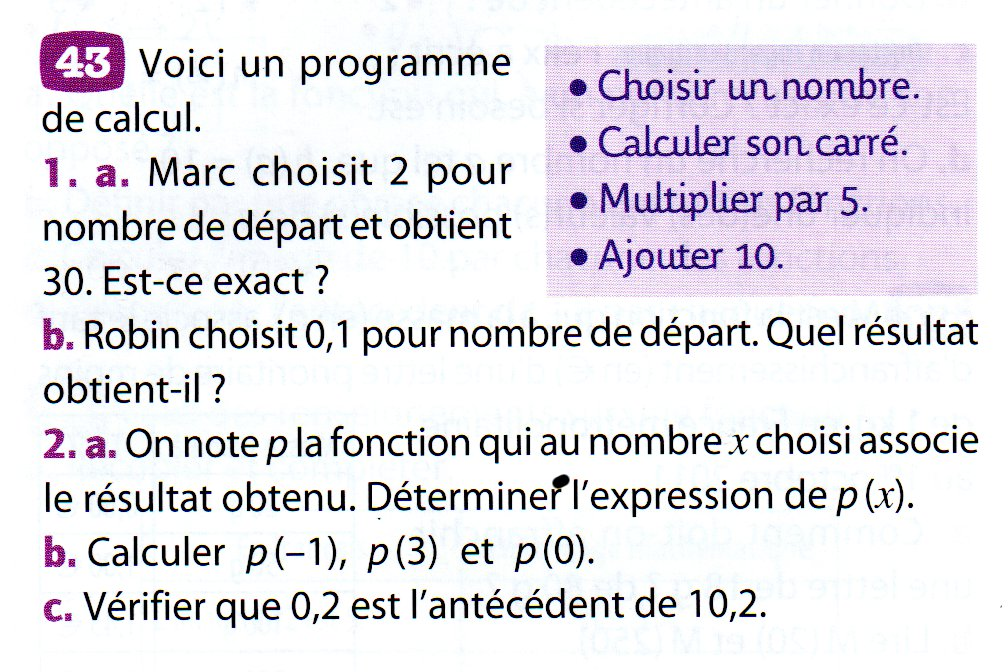
\includegraphics[width=8cm]{images/ex1.jpg}
\end{minipage}
&
\begin{minipage}{9cm}

\ul{Exercice 2:} \textit{(5 points)}

\enskip

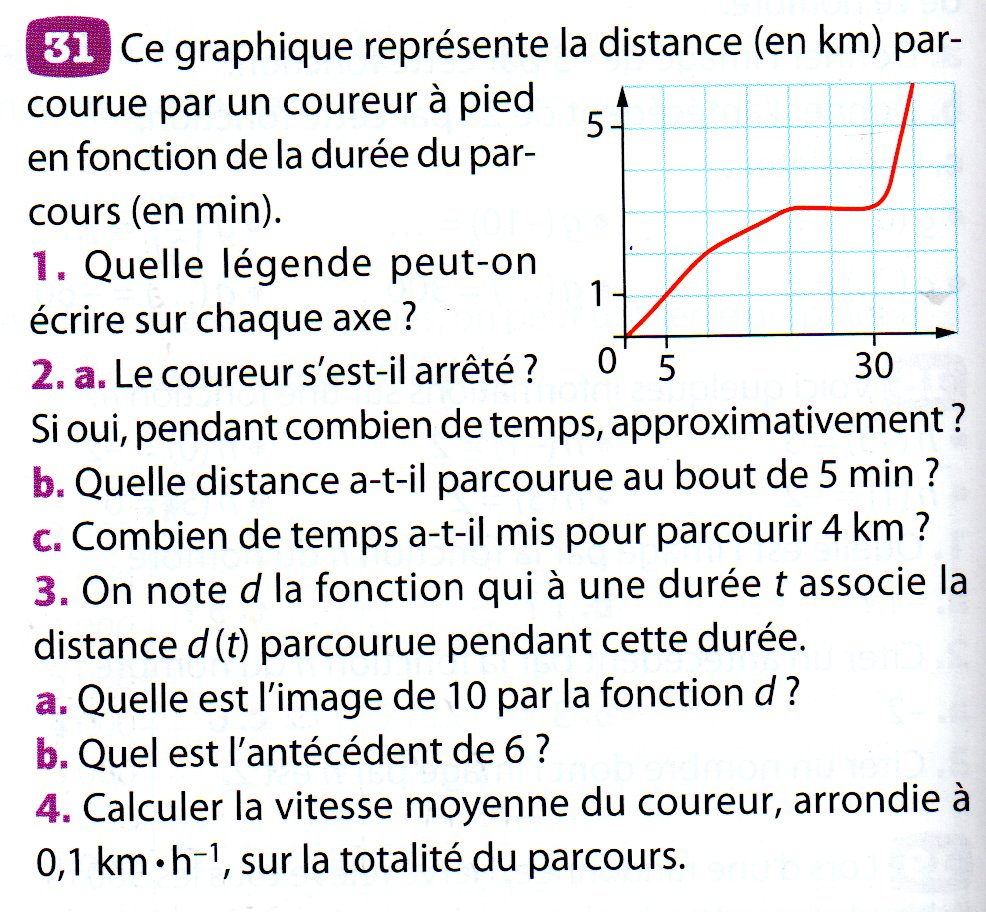
\includegraphics[width=8cm]{images/ex2-fct.jpg}
\end{minipage}
\end{tabular}





\bigskip

\begin{tabular}{cc}
\begin{minipage}{9cm}
\ul{Exercice 3:} \textit{(3 points)}

\enskip

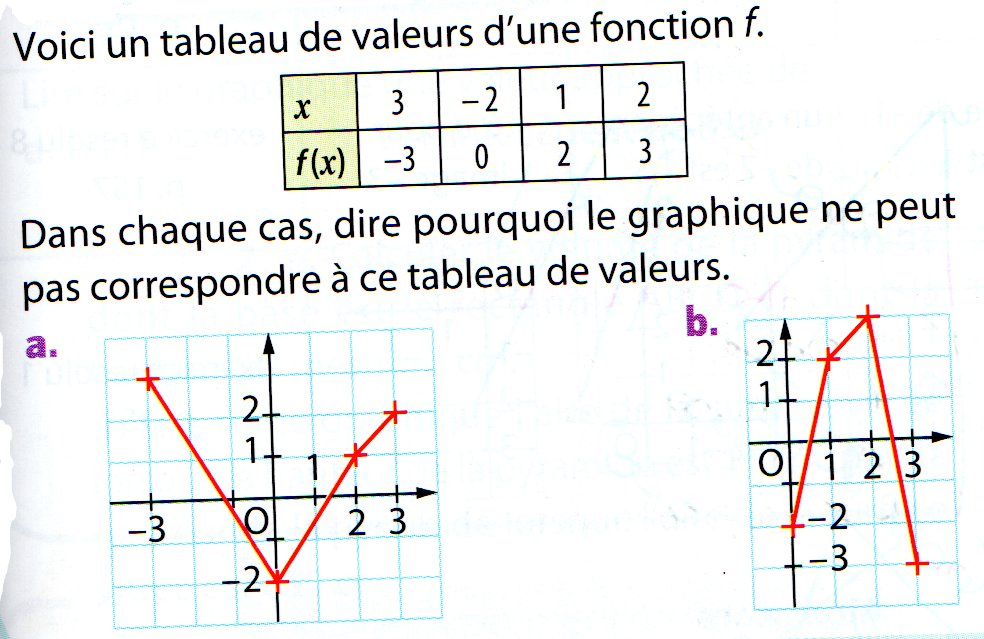
\includegraphics[width=8cm]{images/ex3-fct.jpg}
\end{minipage}
&
\begin{minipage}{10cm}

\ul{Exercice 4:} \textit{(5 points)}


\enskip

Soit $D=(2u+3)^2+(2u+3)(7u-2)$.

\begin{enumerate}
  \item D�velopper puis r�duire D.
  \item Factoriser D.
  \item Calculer D pour $u=-4$.
  \item D�velopper l'expression trouv�e � la question 2. Comparer au r�sultat
  de la question 1.
\end{enumerate}
\end{minipage}
\end{tabular}


\bigskip


\medskip

\ul{Exercice 5:} \textit{(3,5 points)}


\begin{enumerate}
  \item D�velopper et r�duire l'expression $A=(y+1)^2-(y-1)^2$.
  \item Factoriser l'expression A.
  \item Utiliser l'�galit� trouv�e � la premi�re question pour calculer
  $1001^2-999^2$ sans calculatrice.
\end{enumerate}
\bigskip

\ul{Exercice 6:} \textit{(3 points)}

\enskip

Dans la cour d'une ferme, il y a des poules, des moutons et un chien. Le nombre
de poules est �gal au tiers du nombre de moutons. Elsa a compt� les pattes et
en trouve 172. Combien y a-t-il de moutons et de poules?


\bigskip

\ul{Exercice 7:} \textit{(5 points)}

\begin{tabular}{cc}
\begin{minipage}{10cm}
\begin{enumerate}
  \item Construire une r�duction A'B'C'D' du parall�logramme ABCD de rapport
  0,4.
  \item Calculer l'aire de ABCD.
  \item En d�duire l'aire de A'B'C'D'.
\end{enumerate}
\end{minipage}
& 
\begin{minipage}{9cm}
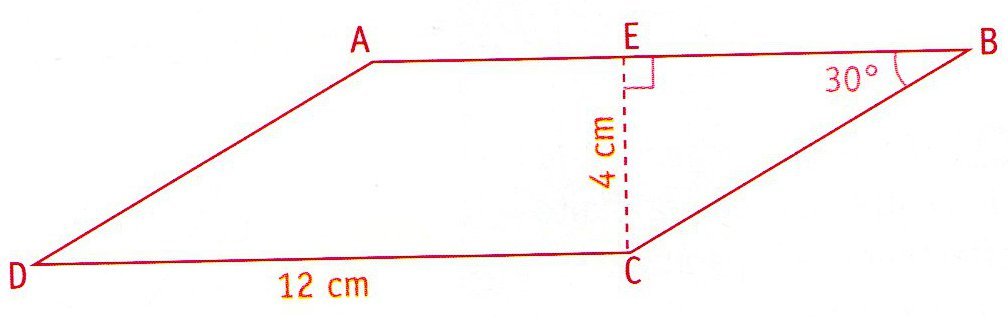
\includegraphics[width=8cm]{images/ex7.jpg}
\end{minipage}
\end{tabular}

\end{document}
